\documentclass[a4paper]{article}
\usepackage[ruled]{algorithm2e}
\usepackage{fullpage} % Package to use full page
\usepackage{parskip} % Package to tweak paragraph skipping
\usepackage{tikz} % Package for drawing
\usepackage{amsmath}
\usepackage{hyperref}
\usepackage{amsfonts}

\title{Report for Computer Project of Applied Stochastic Analysis---Problem 7}
\author{Liangyu Zhang \\ \\ ID:1500010720}
\linespread{1.5}
\begin{document}

\maketitle

\section{Problem Setup}

Consider the following combined Dirichlet-Possion problem:
\begin{displaymath}
\begin{aligned}
    b \nabla u + \frac{1}{2}\Delta u &= f(x, y),\ (x,y)\in B_1(0)\\
    u &= \frac{1}{2}\ \text{on}\ (x,y)\in \mathcal{S}^1
\end{aligned}
\end{displaymath}
, where $b=(x, y)$, $f(x, y) = x^2 + y^2 + 1$. We would like to solve this PDE numerically via the simulation of SDEs.

\section{Detailed Solution}
Let $L$ denote a semi-elliptic partial differential operator on $C^2(\mathbb{R} ^n)$ of the form
\begin{displaymath}
L=\sum_{i=1}^n b_i(x)\frac{\partial}{\partial x_i} + \sum_{i,j=1}^n a_{ij}(x)\frac{\partial ^2}{\partial x_i \partial x_j}
\end{displaymath}
. Then we may rewrite the original PDE as:
\begin{displaymath}
\begin{aligned}
Lu &= -g\ \text{in}\ B_1(0)\\
u &= \phi\ \text{on}\ \mathcal{S}^1
\end{aligned}
\end{displaymath}
where $b=(x,y)^T$, $[a_{ij}]=\frac{1}{2} I_2$, $g=-(x^2+y^2+1)$, $\phi = \frac{1}{2}$. Now consider an Ito diffusion$\{(X_t, Y_t)\}$ whose generator $A$ coincides with $L$ on $C_0^2(\mathbb{R}^2)$. To achieve this we simply choose $b=(x,y)$ and $\sigma = I_2$. According to \textbf{Theorem 9.3.3} in \cite{oksendal2003stochastic}, the solution of the concerned PDE can be represented as:
\begin{displaymath}
u(x,y)=\frac{1}{2}-E^{(x,y)}[\int_0^{\tau_D}(X_s^2+Y_s^2+1)ds]
\end{displaymath}
,where $\tau_D$ is the exit time. Since we have the fact that $E^x(\tau_D)<\infty$ (as shown in prof.Li's lecture notes) and $g(x, y)=-(x^2+y^2+1)$ is bounded in $B_1(0)$, it's then trivial to verify that $E^{(x,y)}[\int_0^{\tau_D}(X_s^2+Y_s^2+1)ds]<\infty$.

With the discussion above, to evaluate the solution of the PDE at some point, say, $(x_0, y_0)$, we just need to compute $E^{(x,y)}[\int_0^{\tau_D}(X_s^2+Y_s^2+1)ds]$. Here we use the standard Euler-Maruyama scheme to simulate the Ito diffusion $\{X_t, Y_t\}$, and then approximate the integral with the simulated track. And the operation described above would be performed multiple times as to estimate the expectation. Detailed algorithm is shown as follows:

\begin{algorithm}
\DontPrintSemicolon % Some LaTeX compilers require you to use \dontprintsemicolon instead
\KwIn{$(x_0,y_0),\ \delta t\ \text{as the step length}$}
\KwOut{$\hat u(x_0, y_0)$}
$sum \gets 0$\;
$i \gets 0$\;
\While{$i < N$}{
  $X_0 \gets x_0$\;
  $Y_0 \gets y_0$\;
  \While{\textbb{True}}{
    $X_{t+1} \gets X_t + X_t * \delta t + N(0, \sqrt{\delta t})$\;
    $Y_{t+1} \gets Y_t + Y_t * \delta t + N(0, \sqrt{\delta t})$\;
    \If{$X_{t+1}^2+Y_{t+1}^2>1$}{
      $\textbf{break}$\;
    }
  }
  $Int \gets \sum_t (X^2_t + Y^2_t + 1)\delta t$\;
  $Sum \gets Sum + Int$\;
  $i \gets i + 1$
}
\Return $Sum/N$\;
\caption{{\sc Estimation of $u(x_0,y_0)$}}
\end{algorithm}

\section{Numerical Results}
The algorithm is implemented in C++, using a random number generator based on hardware entropy. The numerical results are quite satisfactory. Compared to the analytical solution $u(x,y)=(x^2 + y^)/2$, the relative error is less than 1\% when we set $\delta t$ to be $10^{-6}$ and $N$ to be 10000. And clearly the error comes from simulating the Ito diffusion by Euler-Maruyama scheme, estimating the integral by finite sum and approximating the expectation by empirical mean. The numerical convergence order in step length is approximately 1/2, namely, $error\sim\sqrt{\delta t}$, which can be seen from the following picture, where the red line is obtained by performing linear regression to the relative error and square root of step length. 

\begin{figure}[ht]

\centering
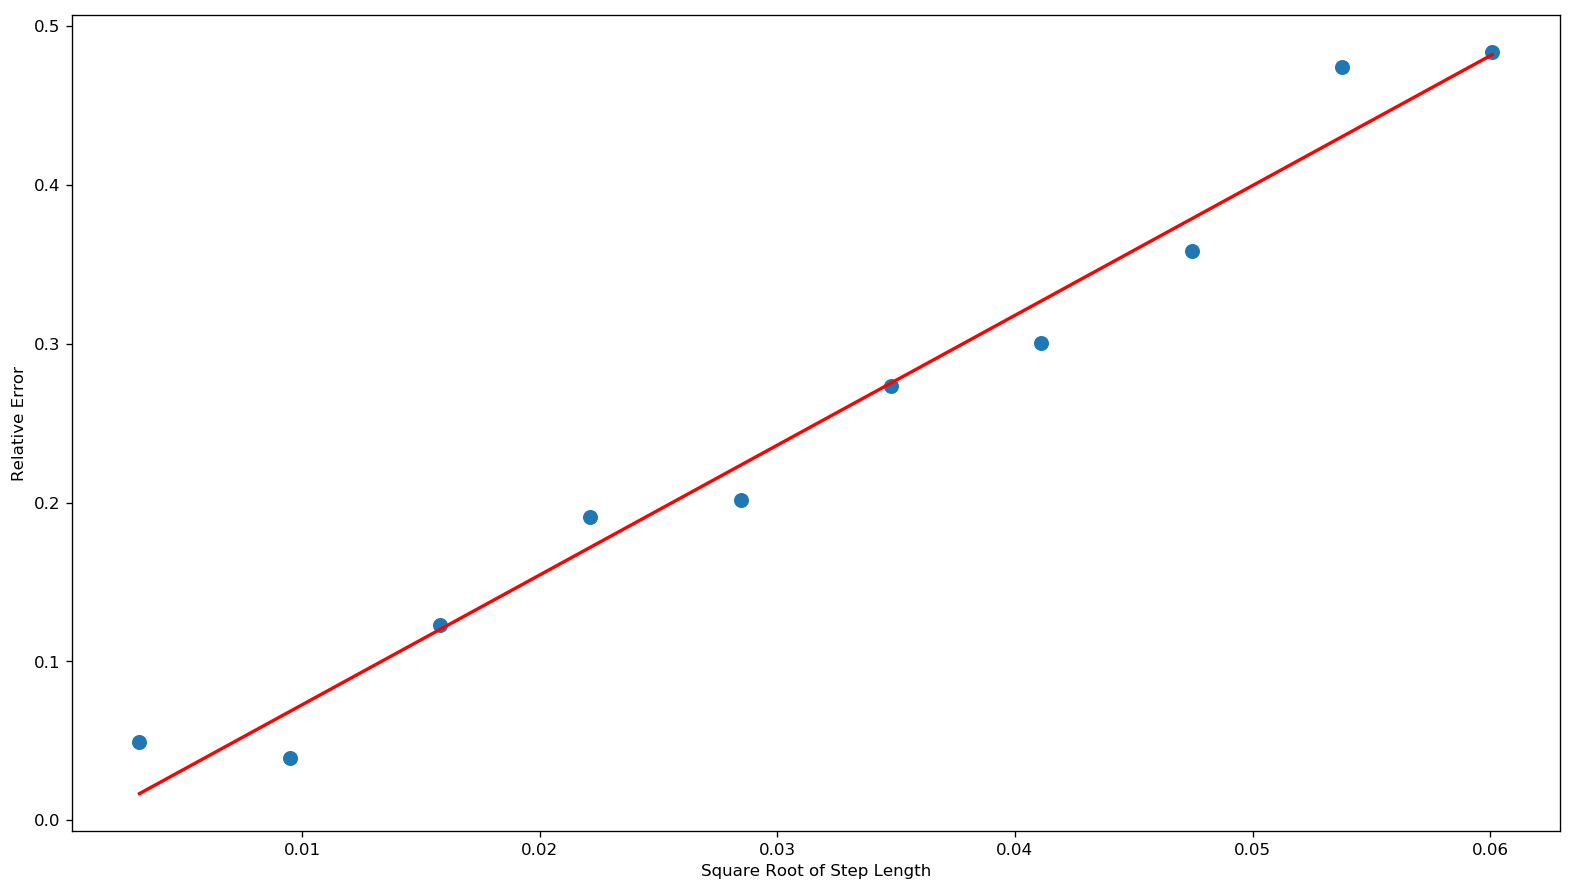
\includegraphics[scale=0.4]{LR.png}

\end{figure}

\bibliographystyle{plain}
\bibliography{bibliography.bib}
\end{document}